\chapter{L'effort et les besoins énergétiques du corps}\label{ch:g10:exercise-and-energy}

Une cycliste sur un vélo de laboratoire pédale contre un frein qui
mesure sa puissance~: \qty{100}{W}, puis \qty{150}{W}, puis
\qty{200}{W}. Un masque sur son visage envoie chaque souffle à un
analyseur. Les nombres à l'écran montent au rythme du frein~: plus elle
fournit de travail mécanique, plus elle consomme d'oxygène et plus elle
rejette de dioxyde de carbone. Ses muscles font tourner à plein la
respiration du \cref{ch:g10:cell-metabolism}, et l'analyseur en lit le
bilan. Ce chapitre suit l'énergie de l'effort, de l'aliment qui la
fournit à l'oxygène qui la libère.

\section{L'énergie entre, le travail sort}

\begin{definition}[Dépense énergétique]\label{def:g10:exercise-and-energy:expenditure}
La \emph{dépense énergétique}\index{dépense énergétique} du corps, en
joules, est l'énergie totale que ses \omterm{def:g10:cells-common-unit:cell}{cellules} libèrent à partir de
molécules organiques pendant une durée donnée. Divisée par la durée,
c'est une \emph{puissance métabolique}, en watts. Au repos, un adulte
dépense environ \qty{80}{W} --- quelque \qty{7000}{kJ} par jour ---
pour faire battre le cœur, faire travailler le cerveau, tenir la
température à \qty{37}{\celsius} et garder les \omterm{def:g10:cells-common-unit:cell}{cellules} en vie~: c'est
le \emph{\omterm{def:g10:cell-metabolism:metabolism}{métabolisme} de base}. Toute activité s'y ajoute.
\end{definition}

\begin{proposition}[Où va l'énergie]\label{prop:g10:exercise-and-energy:efficiency}
Un muscle au travail ne convertit qu'un quart environ de l'énergie
qu'il libère en travail mécanique~; les trois autres quarts partent en
chaleur. Fournir une puissance mécanique $P$ coûte donc au corps une
puissance métabolique d'environ $4P$ au-dessus du repos~: une cycliste
à \qty{100}{W} sur les pédales dépense quelque \qty{400}{W} dans ses
muscles, et son corps doit évacuer \qty{300}{W} de chaleur --- par la
sueur, pour l'essentiel.
\end{proposition}
\admitted

\begin{example}[Budgets quotidiens]\label{ex:g10:exercise-and-energy:budgets}
Un élève assis en cours, marchant jusqu'au lieu d'étude et dormant
dépense environ \qty{9000}{kJ} par jour~; une heure de football y
ajoute quelque \qty{2500}{kJ}~; une journée en montagne avec un sac,
\qty{15000}{kJ} en tout. Un cycliste sur une étape de montagne dépense
\qty{25000}{kJ}, et ne peut pas manger assez dans la journée pour les
couvrir. L'énergie vient des aliments
(\cref{ch:g10:chemistry-of-life})~: \qty{17}{kJ} par gramme de \omterm{def:g10:chemistry-of-life:families}{glucide}
ou de \omterm{def:g10:chemistry-of-life:families}{protéine}, \qty{38}{kJ} par gramme de \omterm{def:g10:chemistry-of-life:families}{lipide}.
\end{example}

\section{La consommation d'oxygène mesure la dépense énergétique}

\begin{proposition}[L'équivalent énergétique de l'oxygène]\label{prop:g10:exercise-and-energy:oxygen}
Puisque l'énergie de l'effort est libérée par la \omterm{prop:g10:cell-metabolism:respiration}{respiration
cellulaire}, qui consomme de l'oxygène, la consommation d'oxygène du
corps mesure sa \omterm{def:g10:exercise-and-energy:expenditure}{dépense énergétique}~: chaque litre d'oxygène consommé
correspond à environ \qty{20}{kJ} libérés, quel que soit le mélange de
glucose et de \omterm{def:g10:chemistry-of-life:families}{lipides} brûlé. Au repos, une personne consomme environ
\qty{0.25}{L} d'oxygène par minute~; à l'effort, la consommation monte
proportionnellement à la puissance fournie, jusqu'à un plafond propre à
chacun.
\end{proposition}
\begin{proof}[Faits expérimentaux]
L'équation de la respiration du \cref{ch:g10:cell-metabolism} donne
\qty{2870}{kJ} pour \qty{6}{mol} d'oxygène, soit \qty{478}{kJ} par
mole, et une mole de gaz occupe environ \qty{24}{L}~: \qty{20}{kJ} par
litre. Pour les \omterm{def:g10:chemistry-of-life:families}{lipides}, le chiffre est \qty{19.6}{kJ/L}, pour les
\omterm{def:g10:chemistry-of-life:families}{glucides} \qty{21.1}{kJ/L}, si bien que le mélange ne change presque
rien. Les mesures en chambre fermée, où la chaleur libérée par un sujet
est recueillie directement, s'accordent au chiffre tiré de l'oxygène à
quelques pour cent près.
\end{proof}

\begin{omfigure}
\begin{tikzpicture}
\begin{axis}[
  width=0.86\linewidth, height=5.8cm,
  axis x line=bottom, axis y line=left,
  xmin=0, xmax=320, ymin=0, ymax=4.2,
  xlabel={puissance mécanique (W)}, ylabel={$\mathrm{O_2}$ consommé (L/min)},
  xlabel style={font=\small, at={(axis description cs:0.5,-0.12)}, anchor=north},
  ylabel style={font=\small},
  tick label style={font=\small},
  xtick={0,50,100,150,200,250,300}, ytick={0,1,2,3,4},
  clip=false,
]
\addplot[thick, omThm, mark=*, mark size=1.6pt] coordinates
  {(0,0.3) (50,0.9) (100,1.5) (150,2.1) (200,2.7) (250,3.2) (300,3.3)};
\draw[dashed, gray] (axis cs:0,3.3) -- (axis cs:320,3.3);
\node[font=\small, anchor=south east] at (axis cs:318,3.32) {$\dot V\!\mathrm{O_2}$max};
\node[font=\small, anchor=south west, align=left] at (axis cs:40,3.42) {pente~: \qty{12}{mL} d'$\mathrm{O_2}$ par minute\\ et par watt};
\end{axis}
\end{tikzpicture}

{\small Consommation d'oxygène d'un sujet pédalant à puissance
croissante. La montée est linéaire --- environ \qty{12}{mL} d'oxygène
par minute et par watt --- jusqu'à ce que la consommation atteigne son
plafond, la $\dot V\!\mathrm{O_2}$max du sujet~; au-delà, le surcroît
de puissance est fourni sans oxygène et ne peut pas durer.}
\end{omfigure}

\begin{definition}[Consommation maximale d'oxygène]\label{def:g10:exercise-and-energy:vo2max}
La \emph{consommation maximale d'oxygène}\index{consommation maximale d'oxygène},
notée $\dot V\!\mathrm{O_2}$max, est le débit le plus élevé auquel le
corps d'une personne peut prélever et utiliser l'oxygène, en litres par
minute --- ou, pour comparer des personnes de tailles différentes, en
millilitres par minute et par kilogramme de masse corporelle. Elle fixe
la plus grande puissance que la respiration seule peut soutenir.
Valeurs typiques~: \qty{35}{mL/min} par kilogramme chez un adulte
sédentaire, \num{50} chez un élève entraîné, \num{80} ou plus chez un
champion d'endurance.
\end{definition}

\begin{example}[Lire la courbe]\label{ex:g10:exercise-and-energy:reading}
Sur la figure, \qty{100}{W} de pédalage coûtent \qty{1.5}{L/min}
d'oxygène~: $1.5 \times 20 = \qty{30}{kJ}$ par minute, soit
\qty{500}{W} de puissance métabolique --- les \qty{100}{W} de travail
plus \qty{400}{W} de chaleur et de besoins de repos, conformément à la
\cref{prop:g10:exercise-and-energy:efficiency}. Le plafond de
\qty{3.3}{L/min} pour un sujet de \qty{66}{kg} vaut \qty{50}{mL/min}
par kilogramme.
\end{example}

\begin{omfigure}
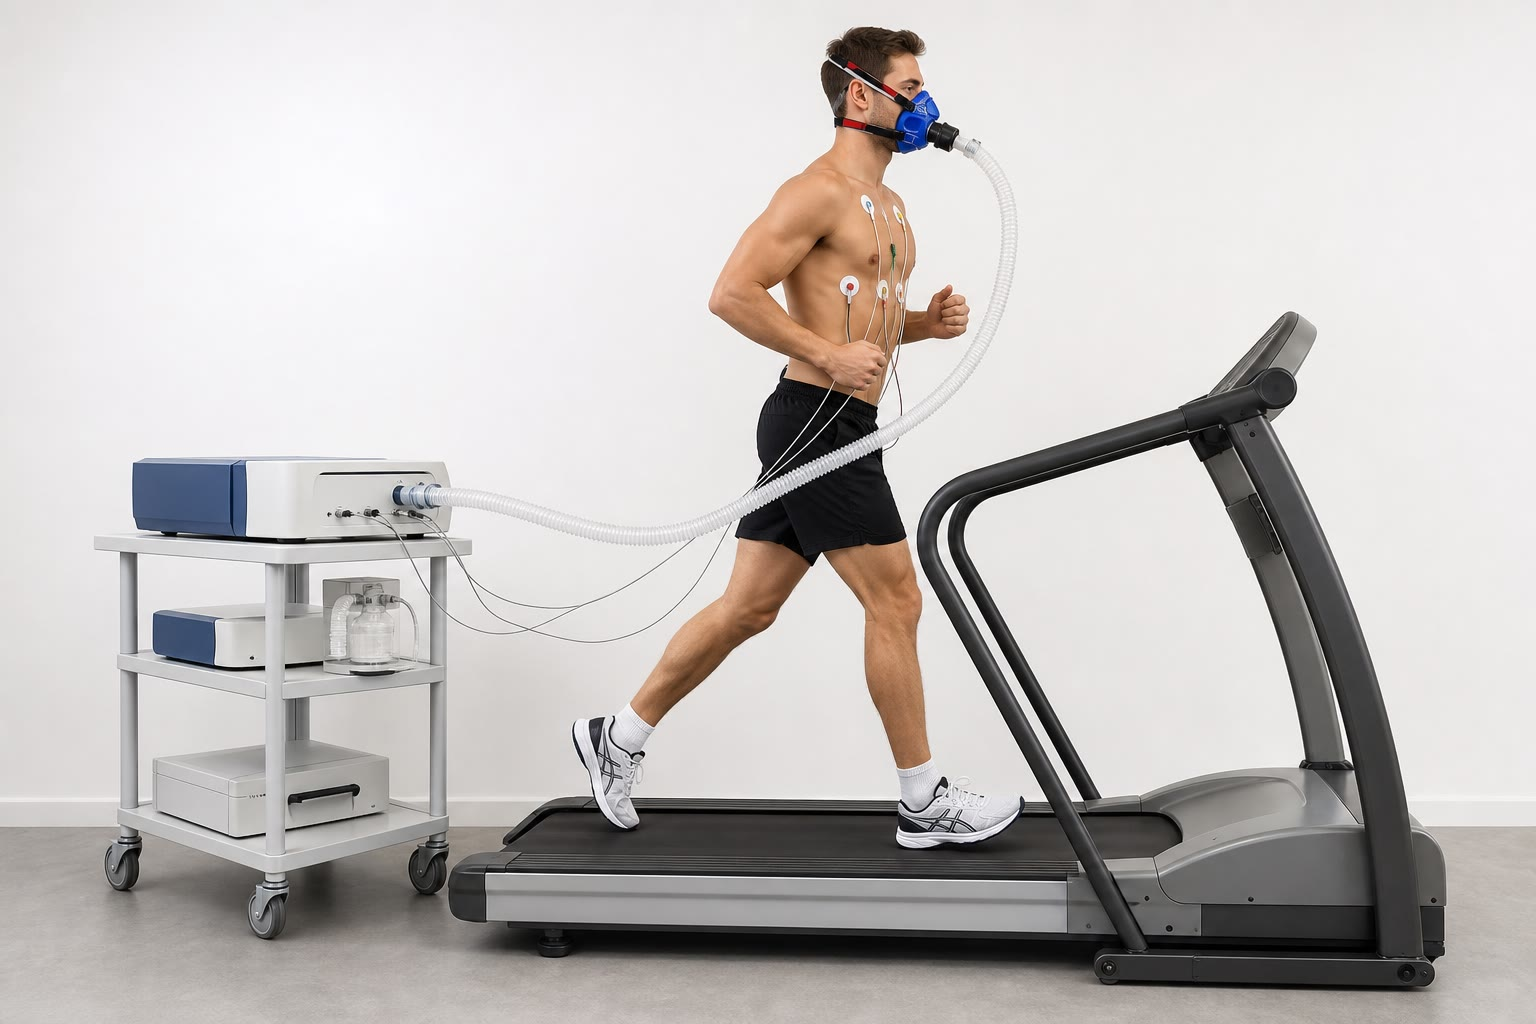
\includegraphics[width=0.62\linewidth]{images/book2/ai/g10-exercise-treadmill-mask.jpg}

{\small Mesurer la consommation d'oxygène à l'effort~: chaque souffle
passe par le masque jusqu'à un analyseur de gaz qui enregistre
l'oxygène prélevé et le dioxyde de carbone rejeté, minute par minute,
tandis que le tapis roulant fixe la puissance.}
\end{omfigure}

\section{Les carburants du muscle}

\begin{proposition}[Trois sources d'ATP]\label{prop:g10:exercise-and-energy:fuels}
La contraction musculaire se paie en ATP, et la \omterm{def:g10:cells-common-unit:cell}{cellule} n'en garde que
pour quelques secondes. Il est renouvelé par trois voies, chacune avec
sa vitesse et sa capacité propres~:
\begin{itemize}
  \item une petite réserve d'un composé phosphaté dans le muscle, qui
        reforme l'ATP instantanément mais dure une dizaine de secondes
        --- le sprint~;
  \item la \omterm{def:g10:cell-metabolism:fermentation}{fermentation} lactique du glucose dans le \omterm{def:g10:cells-common-unit:cell}{cytoplasme},
        rapide mais dispendieuse, qui soutient un effort maximal une à
        deux minutes en produisant de l'acide lactique~;
  \item la \omterm{prop:g10:cell-metabolism:respiration}{respiration cellulaire} dans les \omterm{def:g10:cells-common-unit:organelle}{mitochondries}, plus lente à
        atteindre son plein régime mais de durée presque illimitée, qui
        brûle le glucose du sang, le \omterm{def:g10:exercise-and-energy:glycogen}{glycogène} du muscle et les acides
        gras des graisses du corps.
\end{itemize}
La part de chacune dépend de l'intensité et de la durée de l'effort.
\end{proposition}
\admitted

\begin{omfigure}
\begin{tikzpicture}
\begin{axis}[
  ybar stacked, bar width=18pt,
  width=0.86\linewidth, height=5.6cm,
  axis x line=bottom, axis y line=left,
  ymin=0, ymax=100, ylabel={part de l'énergie (\%)}, ylabel style={font=\small},
  symbolic x coords={10 s, 1 min, 4 min, 30 min, 2 h},
  xtick=data, tick label style={font=\small},
  xlabel={durée d'un effort maximal},
  xlabel style={font=\small, at={(axis description cs:0.5,-0.12)}, anchor=north},
  enlarge x limits=0.15,
  legend style={at={(0.5,-0.3)}, anchor=north, legend columns=3,
                font=\small, draw=none},
]
\addplot[fill=omThm!50, draw=omThm] coordinates {(10 s,85) (1 min,25) (4 min,8) (30 min,2) (2 h,1)};
\addplot[fill=omProp!50, draw=omProp] coordinates {(10 s,12) (1 min,50) (4 min,32) (30 min,8) (2 h,2)};
\addplot[fill=omDef!50, draw=omDef] coordinates {(10 s,3) (1 min,25) (4 min,60) (30 min,90) (2 h,97)};
\legend{réserve phosphatée, fermentation lactique, respiration}
\end{axis}
\end{tikzpicture}

{\small Part approchée des trois sources d'ATP dans un effort maximal
de durée donnée. Un 100 mètres tourne sur la réserve phosphatée~; un
400 mètres, largement sur la \omterm{def:g10:cell-metabolism:fermentation}{fermentation}~; tout ce qui dépasse
quelques minutes, sur la respiration.}
\end{omfigure}

\begin{definition}[Glycogène]\label{def:g10:exercise-and-energy:glycogen}
Le \emph{glycogène}\index{glycogène} est la forme animale de réserve
glucidique~: une chaîne ramifiée d'unités de glucose, conservée en
granules dans les \omterm{def:g10:cells-common-unit:cell}{cellules} musculaires (environ \qty{400}{g} chez un
adulte) et dans le foie (environ \qty{100}{g}). Le glycogène musculaire
alimente le muscle qui le stocke~; le glycogène du foie est dégradé en
glucose libéré dans le sang, ce qui maintient la glycémie près de
\qty{1}{g/L} pour le cerveau et les autres tissus. La graisse, stockée
dans les \omterm{def:g10:cells-common-unit:cell}{cellules} adipeuses, est la réserve bien plus vaste
(\cref{ch:g10:chemistry-of-life}), mais elle ne peut être brûlée que
lentement et seulement avec de l'oxygène.
\end{definition}

\begin{example}[Le mur du marathon]\label{ex:g10:exercise-and-energy:wall}
La course consomme environ \qty{4}{kJ} par kilogramme de masse
corporelle et par kilomètre~; un coureur de \qty{70}{kg} dépense
\qty{280}{kJ/km}, et un marathon coûte \qty{11800}{kJ}. Les réserves de
\omterm{def:g10:exercise-and-energy:glycogen}{glycogène} en détiennent environ \qty{8500}{kJ}. Si le coureur brûle son
\omterm{def:g10:exercise-and-energy:glycogen}{glycogène} trop vite, les réserves s'épuisent vers le trentième
kilomètre~; les muscles doivent alors compter sur la graisse, qui
fournit l'énergie à peine à la moitié du débit, et l'allure
s'effondre --- c'est «~le mur~». Les coureurs entraînés brûlent une
part plus grande de graisse dès le départ, et mangent des \omterm{def:g10:chemistry-of-life:families}{glucides} en
course.
\end{example}

\begin{omfigure}
\begin{tikzpicture}[>=Stealth, font=\small,
  b/.style={draw, rounded corners, align=center, minimum height=0.9cm, text width=2.5cm}]
  \node[b, fill=omDef!12] (food) at (0,2.2) {aliments~:\\ glucides, lipides};
  \node[b, fill=omDef!12] (gly) at (0,0.6) {glycogène (muscle,\\ foie), glucose sanguin};
  \node[b, fill=omDef!12] (fat) at (0,-1.0) {acides gras des\\ graisses du corps};
  \node[b, fill=omThm!12, minimum height=2.6cm] (mit) at (4.3,-0.2) {mitochondries~:\\ respiration};
  \node[b, fill=omProp!15] (o2) at (4.3,2.2) {oxygène, venu des\\ poumons et du sang};
  \node[b, fill=omMeth!15] (atp) at (9.2,-0.2) {ATP};
  \node[b, fill=white] (work) at (12.5,0.8) {travail musculaire\\ (environ 25\%)};
  \node[b, fill=white] (heat) at (12.5,-1.2) {chaleur\\ (environ 75\%)};
  \draw[->] (food) -- (gly);
  \draw[->] (food.west) to[bend right=40] (fat.west);
  \draw[->] (gly) -- (mit);
  \draw[->] (fat) -- (mit);
  \draw[->] (o2) -- (mit);
  \draw[->] (mit) -- node[above, font=\scriptsize] {$\mathrm{CO_2}$ sortant} (atp);
  \draw[->] (atp) -- (work);
  \draw[->] (atp) -- (heat);
\end{tikzpicture}

{\small La chaîne énergétique de l'effort prolongé~: des carburants
venus des aliments et des réserves du corps, de l'oxygène venu de la
respiration, de l'ATP fabriqué dans les \omterm{def:g10:cells-common-unit:organelle}{mitochondries} et dépensé pour
la contraction --- les trois quarts partant en chaleur.}
\end{omfigure}

\section{Mesurer et raisonner}

\begin{method}[Un calcul d'énergie à l'effort]\label{met:g10:exercise-and-energy:calc}
\begin{enumerate}
  \item À partir de l'oxygène~: énergie (\unit{kJ}) $=$ oxygène
        consommé (\unit{L}) $\times 20$. Retrancher la consommation de
        repos si la question demande le coût du seul effort.
  \item À partir de la puissance mécanique~: puissance métabolique
        $\approx 4 P$~; énergie $=$ puissance $\times$ durée
        (\qty{1}{W} pendant \qty{1}{s} fait \qty{1}{J}~; \qty{1}{kWh}
        $= \qty{3600}{kJ}$).
  \item À partir du carburant~: masse brûlée $=$ énergie $/$ valeur
        énergétique (\qty{17}{kJ/g} pour les \omterm{def:g10:chemistry-of-life:families}{glucides}, \qty{38}{kJ/g}
        pour les \omterm{def:g10:chemistry-of-life:families}{lipides})~; le \omterm{def:g10:exercise-and-energy:glycogen}{glycogène} est stocké avec trois fois sa
        masse d'eau.
  \item Vérifier les ordres de grandeur~: une journée entière fait
        environ \qty{10000}{kJ}~; une heure difficile,
        \qtyrange{2000}{3000}{kJ}~; un marathon, \qty{12000}{kJ}.
\end{enumerate}
\end{method}

\begin{example}[Une heure de vélo]\label{ex:g10:exercise-and-energy:hour}
Une heure à \qty{150}{W} sur les pédales~: puissance métabolique
d'environ \qty{600}{W}, énergie $600 \times 3600 = \qty{2.16e6}{J} \approx
\qty{2200}{kJ}$~; oxygène $2200/20 = \qty{110}{L}$, soit
\qty{1.8}{L/min} --- en accord avec la courbe. Si la moitié vient des
\omterm{def:g10:chemistry-of-life:families}{glucides}~: $1100/17 \approx \qty{65}{g}$ de glucose ou de \omterm{def:g10:exercise-and-energy:glycogen}{glycogène}, et
$1100/38 \approx \qty{29}{g}$ de graisse.
\end{example}

\begin{remark}[Pourquoi l'oxygène doit arriver]\label{rem:g10:exercise-and-energy:delivery}
Tout ce qui précède suppose que l'oxygène parvient aux \omterm{def:g10:cells-common-unit:organelle}{mitochondries}
aussi vite qu'elles peuvent l'utiliser. C'est le rôle des poumons, du
cœur et du sang, dont la réponse à l'effort --- respiration plus
rapide, battements plus rapides et plus forts, sang redirigé vers les
muscles --- fait l'objet du \cref{ch:g10:heart-lungs-effort}. La
$\dot V\!\mathrm{O_2}$max est surtout une limite de livraison, non
d'appétit des muscles.
\end{remark}

\section{Exercices}

\begin{exercise}[$\star$]\label{exo:g10:exercise-and-energy:1}
Définir le \omterm{def:g10:cell-metabolism:metabolism}{métabolisme} de base et donner son ordre de grandeur en watts
et en kilojoules par jour.
\end{exercise}

\begin{exercise}[$\star$]\label{exo:g10:exercise-and-energy:2}
Un sujet consomme \qty{2.0}{L} d'oxygène par minute. Quelle est sa
\omterm{def:g10:exercise-and-energy:expenditure}{dépense énergétique} en kilojoules par minute, et en watts~?
\end{exercise}

\begin{exercise}[$\star$]\label{exo:g10:exercise-and-energy:3}
Nommer les trois voies par lesquelles un muscle renouvelle son ATP et
donner la durée typique que chacune peut soutenir à elle seule.
\end{exercise}

\begin{exercise}[$\star$]\label{exo:g10:exercise-and-energy:4}
Qu'est-ce que la $\dot V\!\mathrm{O_2}$max~? Convertir \qty{3.5}{L/min}
pour un sujet de \qty{70}{kg} en millilitres par minute et par
kilogramme.
\end{exercise}

\begin{exercise}[$\star$]\label{exo:g10:exercise-and-energy:5}
Où le \omterm{def:g10:exercise-and-energy:glycogen}{glycogène} est-il stocké, en quelles quantités, et à quoi sert
chaque réserve~?
\end{exercise}

\begin{exercise}[$\star\star$]\label{exo:g10:exercise-and-energy:6}
Sur la figure oxygène--puissance, lire la consommation d'oxygène à
\qty{200}{W} et calculer la puissance métabolique. En déduire la
chaleur produite par seconde.
\end{exercise}

\begin{exercise}[$\star\star$]\label{exo:g10:exercise-and-energy:7}
Une randonneuse de \qty{60}{kg} monte de \qty{800}{m} en deux heures.
Calculer le travail mécanique contre la pesanteur
($g = \qty{9.8}{N/kg}$), l'énergie dépensée par ses muscles si le
rendement est de 25~\%, et la puissance métabolique moyenne au-dessus
du repos.
\end{exercise}

\begin{exercise}[$\star\star$]\label{exo:g10:exercise-and-energy:8}
À l'aide de la figure en barres empilées, expliquer pourquoi un coureur
de 400 mètres est essoufflé et endolori à l'arrivée alors qu'un
sprinteur de 100 mètres souffle à peine.
\end{exercise}

\begin{exercise}[$\star\star$]\label{exo:g10:exercise-and-energy:9}
Une athlète dépense \qty{3000}{kJ} au cours d'une séance
d'entraînement, dont 60~\% venant des \omterm{def:g10:chemistry-of-life:families}{glucides}. Quelle masse de
\omterm{def:g10:exercise-and-energy:glycogen}{glycogène} a-t-elle utilisée, et quelle masse d'eau a été libérée avec
lui~?
\end{exercise}

\begin{exercise}[$\star\star$]\label{exo:g10:exercise-and-energy:10}
Une tablette de chocolat de \qty{50}{g} fournit \qty{1100}{kJ}.
Pendant combien de temps ferait-elle avancer un cycliste pédalant à
\qty{150}{W}~?
\end{exercise}

\begin{exercise}[$\star\star$]\label{exo:g10:exercise-and-energy:11}
Pourquoi la température du corps monte-t-elle à l'effort, et par quel
mécanisme l'empêche-t-on de monter davantage~?
\end{exercise}

\begin{exercise}[$\star\star\star$]\label{exo:g10:exercise-and-energy:12}
Deux sujets de \qty{60}{kg} et \qty{90}{kg} ont tous deux une
$\dot V\!\mathrm{O_2}$max de \qty{3.6}{L/min}. Lequel peut courir le
plus vite en montée, et lequel peut pédaler le plus fort à plat sur un
vélo de laboratoire~? Expliquer.
\end{exercise}

\begin{exercise}[$\star\star\star$]\label{exo:g10:exercise-and-energy:13}
La consommation d'oxygène d'un coureur pendant une course est de
\qty{3.0}{L/min} à une allure qui, d'après la courbe, exigerait
\qty{3.4}{L/min}. D'où vient la différence, et que ressentira le
coureur après quelques minutes~?
\end{exercise}

\begin{exercise}[$\star\star\star$]\label{exo:g10:exercise-and-energy:14}
Expliquer, à l'aide des trois voies de renouvellement de l'ATP,
pourquoi on ne perd pas de graisse aussi efficacement en s'exerçant à
intensité maximale par courtes salves qu'en s'exerçant modérément
longtemps.
\end{exercise}

\begin{exercise}[$\star\star\star$]\label{exo:g10:exercise-and-energy:15}
Une cycliste sur une étape de montagne dépense \qty{25000}{kJ} dans la
journée. Son \omterm{def:g10:exercise-and-energy:glycogen}{glycogène} en détient \qty{8500}{kJ} et elle mange
\qty{6000}{kJ} pendant l'étape. Estimer la masse de graisse corporelle
qu'elle brûle, et expliquer pourquoi les coureurs mangent sans cesse
sur une telle étape.
\end{exercise}

\section{Problème~: où se dresse le mur}

\begin{problem}[{Problème du week-end --- le bilan énergétique d'un
marathon~: l'oxygène que la coureuse respire, le glycogène qu'elle
porte, le kilomètre où il s'épuise, et ce que change l'entraînement}]
\label{pb:g10:exercise-and-energy:1}
Nadia, \qty{60}{kg}, court un marathon (\qty{42.2}{km}) en
\qty{3}{h}\,\qty{30}{min}. La course coûte \qty{4.0}{kJ} par kilogramme
et par kilomètre. Ses muscles détiennent \qty{300}{g} de \omterm{def:g10:exercise-and-energy:glycogen}{glycogène} et
son foie \qty{80}{g}~; le \omterm{def:g10:exercise-and-energy:glycogen}{glycogène} et le glucose donnent
\qty{17}{kJ/g}, la graisse \qty{38}{kJ/g}~; un litre d'oxygène libère
\qty{20}{kJ}. Sa $\dot V\!\mathrm{O_2}$max vaut \qty{52}{mL/min} par
kilogramme.

\medskip
\noindent\textbf{Partie I --- Le coût de la course.}
\begin{enumerate}
  \item Calculer le coût énergétique du marathon pour Nadia.
  \item Calculer sa puissance métabolique moyenne pendant la course,
        en watts.
  \item Calculer le volume d'oxygène qu'elle consomme sur la course,
        puis sa consommation d'oxygène moyenne en litres par minute.
  \item Exprimer cette consommation en millilitres par minute et par
        kilogramme, et en pourcentage de sa
        $\dot V\!\mathrm{O_2}$max.
  \item Sa consommation de repos vaut \qty{0.2}{L/min}. Quelle
        fraction de sa consommation du jour de course la course
        elle-même représente-t-elle~?
\end{enumerate}

\medskip
\noindent\textbf{Partie II --- Les réserves.}
\begin{enumerate}[resume]
  \item Calculer l'énergie détenue dans ses réserves de \omterm{def:g10:exercise-and-energy:glycogen}{glycogène}.
  \item Si elle ne brûlait que du \omterm{def:g10:exercise-and-energy:glycogen}{glycogène}, à quel kilomètre les
        réserves s'épuiseraient-elles~?
  \item En réalité, elle brûle un mélange~: 80~\% de \omterm{def:g10:chemistry-of-life:families}{glucides}, 20~\%
        de graisse à son allure de course. À quel kilomètre le
        \omterm{def:g10:exercise-and-energy:glycogen}{glycogène} s'épuise-t-il alors~?
  \item Quelle masse de graisse brûle-t-elle dans la course~? Comparer
        aux \qty{9}{kg} de graisse que porte habituellement une femme
        de \qty{60}{kg}.
  \item Expliquer, à partir de la
        \cref{prop:g10:exercise-and-energy:fuels}, pourquoi elle ne
        peut pas simplement brûler de la graisse seule une fois le
        \omterm{def:g10:exercise-and-energy:glycogen}{glycogène} épuisé et garder la même allure.
\end{enumerate}

\medskip
\noindent\textbf{Partie III --- Battre le mur.}
\begin{enumerate}[resume]
  \item Pendant la course, elle boit une solution sucrée qui fournit
        \qty{60}{g} de \omterm{def:g10:chemistry-of-life:families}{glucides} par heure. Quelle énergie cela
        ajoute-t-il sur la course, et combien de kilomètres de
        consommation glucidique cela couvre-t-il~?
  \item Refaire la question 8 avec la boisson. Finit-elle désormais
        avant que le \omterm{def:g10:exercise-and-energy:glycogen}{glycogène} ne s'épuise~?
  \item Trois jours avant la course, elle fait une «~surcharge~»
        glucidique et porte son \omterm{def:g10:exercise-and-energy:glycogen}{glycogène} musculaire à \qty{500}{g}.
        Chaque gramme est stocké avec \qty{3}{g} d'eau. De combien sa
        masse augmente-t-elle, et ce que cela coûte en énergie par
        kilomètre~?
  \item L'entraînement fait passer son mélange d'allure de course à
        55~\% de \omterm{def:g10:chemistry-of-life:families}{glucides} et 45~\% de graisse. Avec la surcharge et la
        boisson, à quel kilomètre le \omterm{def:g10:exercise-and-energy:glycogen}{glycogène} s'épuiserait-il~?
        Commenter.
  \item Pourquoi le cerveau, qui n'utilise que du glucose, fait-il
        ressentir l'épuisement du \omterm{def:g10:exercise-and-energy:glycogen}{glycogène} comme une fatigue extrême,
        alors que les muscles ont encore de la graisse à brûler~?
\end{enumerate}

\medskip
\noindent\textbf{Partie IV --- Les chiffres d'un champion.}
Un coureur de haut niveau de \qty{55}{kg} court le marathon en
\qty{2}{h}\,\qty{05}{min}, avec un coût de course de \qty{3.6}{kJ} par
kilogramme et par kilomètre et une $\dot V\!\mathrm{O_2}$max de
\qty{80}{mL/min} par kilogramme.
\begin{enumerate}[resume]
  \item Calculer le coût énergétique de la course pour le champion et
        sa consommation d'oxygène moyenne en litres par minute.
  \item Quel pourcentage de sa $\dot V\!\mathrm{O_2}$max
        soutient-il~? Comparer au chiffre de Nadia.
  \item Deux choses distinguent le champion~: un plafond plus haut et
        un coût par kilomètre plus bas. Laquelle des deux est
        l'«~économie de course~»~? Calculer de combien la seule
        différence de coût change l'énergie de la course pour un
        coureur de \qty{55}{kg}.
  \item Ses muscles détiennent \qty{500}{g} de \omterm{def:g10:exercise-and-energy:glycogen}{glycogène} après
        surcharge. À 70~\% de consommation glucidique, atteint-il
        l'arrivée avec cela sans boire~?
  \item Énoncer le résultat~: pour Nadia, le kilomètre où le mur se
        dresse sans préparation, et les trois mesures qui le repoussent
        au-delà de la ligne d'arrivée.
\end{enumerate}
\end{problem}
